\chapter{Curator}
\begin{multicols}{2}

Curating could be described in a very simplistic manner: the organization of time and space between selected works in a museum. However, there is so much more depth and meaning in the curating process- much more than just new works and organization. A curator not only has the benefit of gathering new works, but also receives the pleasure of discovering the method of communication between the art in the given space of an exhibition with the ultimate goal of translating that hidden language to the audience. Curators are given this ultimate power of communication and emotion without having to say a word. They have the responsibility of communicating an artist’s works of deep emotional investment to the audience and ultimately hoping for the audience to feel transformed after an exhibition. As Carson Chan, a recent graduate from Princeton, stated, “Make sure your exhibition requires your audience’s physical presence; for everything else there’s the Internet.” (Sayej) In this technological age, curators have to face the global Internet. Anyone can see a painting or work of art after 15 seconds of searching; therefore, curators have to create an impact on the audience so that it becomes clear that the digital picture will not suffice. 

Museum curators oversee museum collections by managing the acquisition, preservation, and display of museum artifacts (“Art History, Criticism, and Conservation College Degree Programs”). Curators are often required to take record of and preserve works, as well as supervise staff. Public relations, education, and marketing are often included in the job, causing curators to require a variety of skills. Curators are responsible for creating innovative and interesting exhibitions to appeal to the public, taking part in each aspect of the construction. From outlining and assembling works, to figuring out the art of space and juxtaposition on the display wall, a curator is there every step of the way. Curators usually work in a museum, gallery, or historical site. They will often have to negotiate for collections as well as advertise to the public (“Art History, Criticism, and Conservation College Degree Programs”). A bachelor's degree is the minimum education requirement for museum curators, though a master's degree and/or work experience gives job applicants an edge. A PhD is necessary for some higher-level positions. Museum curators are estimated to make around \$50,000 annually (“Art History, Criticism, and Conservation College Degree Programs”).

\end{multicols}

\section{Top Colleges}

\begin{table}[H]
\centering
\caption{Undergraduate Colleges}
\label{Curator Undergraduate Colleges}
\resizebox{\textwidth}{!}{%
\begin{tabular}{llrlr}
\hline
\multicolumn{5}{|l|}{Dream Schools}                                                    \\ \hline
Oxford University          & Total 3 year cost: & \$76,000  & 20 year ROI: & \$923,500 \\
Courtauld Institute of Art & Total 3 year cost: & \$73,500  & 20 year ROI: & \$923,500 \\ \hline
\multicolumn{5}{|l|}{Best Value Schools}                                               \\ \hline
University of Edinburgh    & Total 5 year cost: & \$157,500 & 20 year ROI: & \$842,500 \\
University of Amsterdam    & Total 3 year cost: & \$6,771   & 20 year ROI: & \$993,229
\end{tabular}%
}
\end{table}

\begin{table}[H]
\centering
\caption{Graduate Universities}
\label{Curator Graduate Universities}
\resizebox{\textwidth}{!}{%
\begin{tabular}{llrlr}
\hline
\multicolumn{5}{|l|}{Dream Schools}                                                                \\ \hline
School of the Art Institute of Chicago & Total 3 year cost:  & \$85,320 & 20 year ROI: & \$914,680 \\
Courtauld Institute of Art             & Total 9 month cost: & \$11,880 & 20 year ROI: & \$988,120 \\ \hline
\multicolumn{5}{|l|}{Best Value Schools}                                                           \\ \hline
Nuova Accademia di Belle Arti Milano   & Total 2 year cost:  & \$13,760 & 20 year ROI: & \$986,240 \\
University of Edinburgh                & Total 2 year cost:  & \$12,900 & 20 year ROI: & \$987,100
\end{tabular}%
}
\end{table}

	\begin{Figure}
	 \centering
	 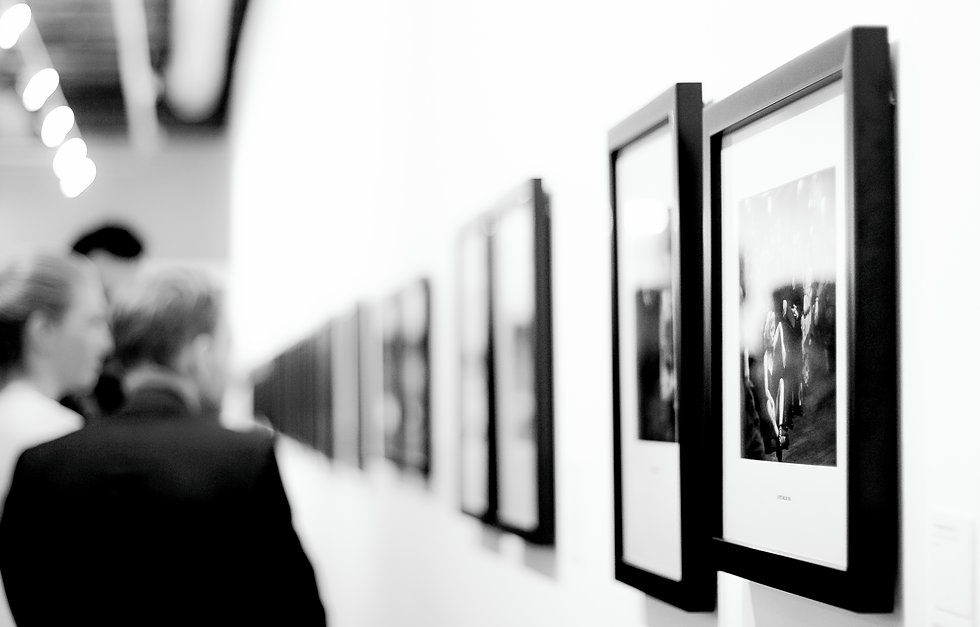
\includegraphics[width=\linewidth]{images/Curator}
	 \captionof{figure}{Curators looking at art (WIX)}
	 \label{fig:Curators looking at art}
	\end{Figure}

\begin{multicols}{2}

\section{Degree Description}
	In order to become a curator, a degree in art history is highly recommended. Art history provides a background of what curators will be working with and will allow the curator to understand the importance of the work he or she is dealing with in exhibitions or collections. Art history is the study of humanity through various works of art (“Art History Basics”). Art History focuses on the questions of why and how, within a specific culture and historical context, specific masterpieces can communicate such strong emotions to the audience. Through studying previous works of art, the student is presented with an unparalleled world view and a massive amount of cultural understanding that wouldn’t be obtained otherwise (“Why Look at Art?”). The materials studied in art history are expanding- along with the traditional works of art such as sculptures, paintings, sketches, and buildings, now new art forms such as film are studied as well, which gives an exciting future for the study of art history (“College and Career Planning”). 

	Most of the undergraduate and graduate programs I have selected are abroad, which varies from the American system of education in a couple ways. In the UK and Europe, universities do not require you to take classes that do not pertain to your major (which has its own pros and cons). Therefore, most of my classes required to get a bachelors in art history are completed in three years instead of four. The curriculums selected in my universities above all require a language study, despite how many languages you already speak, and at least a semester abroad in order to graduate. An important aspect to keep in mind when looking at art history degrees is to see which schools offer a certificate of museology in the bachelors degree, which allows you to work in museums. Some schools have requirements that other schools do not have. For example, at the University of Amsterdam, you are required to obtain some type of teaching position in your third year. In general, the curriculum remains pretty similar. The first year typically covers a broad range of art history and deals with the major themes, and most classes are lectures. In the second year, the curriculum becomes more specialized and really dives into the details of art periods. The second year focuses on the student’s critical analyzation and various approaches to looking at art. In the second semester of the second year, the student chooses two more in-depth classes. In the third and final year, the student chooses two more specialized classes. These are at a more advanced level than second year and prepare students for further study or research. By the end of the third year, the student should get an internship or a sort of work experience relevant to history and/or art in some fashion. 

	Since curatorial positions often require graduate degrees and highly encourage PhDs, most students intending to become curators continue their education. A unique program I have listed under my undergraduate programs is the Fine Arts Masters program at University of Edinburgh. As described on their website, 
	\begin{quote}
		“The Fine Art MA is a five-year degree during which you study both History of Art and Art practice. In Art you are given a broad base in your first year – which includes the study of painting, sculpture, photography, and intermedia – before you go on to focus your work on a particular specialism” (“History of Art - MA (Hons).”). 
	\end{quote}
	This program would allow me to get my masters and bachelors all in one program while residing in one of the art heritage centers of the world. In the graduate programs, such as the last two years in the Edinburgh fine arts program, students start to specialize in a specific area of art, such as impressionism, medieval, modern, etc. Usually the language chosen to study is relevant to the art period, and if the student’s previous language was not relevant to the art period the student is specializing in, the graduate program guides your language studies. For example, if a student was to specialize in French impressionism, he or she would study French. Art curator students have the choice to earn a graduate degree in museum studies, which deals with museum management and conservation. The masters programs I have chosen vary between each curriculum on requirements, but they all require some type of museum work experience, which they help you find. 

\section{Interview}
	Mrs. Esquivel is a recent Art History graduate from Washington University in St. Louis. She graduated with a Bachelors in Design and Architecture and a second Major in Art History. She is applying to Courtauld Institute for their Masters and PhD programs. Gabby graduated in May 2015 and hopes to be a curator in the future. \\ 
	Asked best tips she could give to aspiring curators, she replied with many answers.
	\begin{quote}
		“Don’t rush into your graduate schools. Really at this time in age, all professors want you to work between your undergraduate and masters. Art History and curating is complicated because they want to be selective. You should really specialize in one area, for me, I’m doing modern and contemporary art. Masters is specific field with a 1 on 1 setting. You can be a perfect 4.0 resume student, but if you’re coming straight from undergrad, you won’t get what you’re looking for because schools want you to get experience before you specialize.”
	\end{quote}
	\begin{quote} 
		“From this point, a masters is helpful across the board, but having a PhD is what differentiates academic perspectives. If you want to work in a Museum as a Curator, you basically need your PhD.”
	\end{quote}
	\begin{quote}
		“Languages are super helpful, language study\ldots\ You really have to show profeciency in at least two languages. German is big in modern studies, Italian for any antiquity, and impressionist is most definitely French. Languages corresponds immensely.”
	\end{quote}
	When asked what she thinks of the value of an art history degree in today’s society, Esquivel responded with:
	\begin{quote}
		“In my opinion, I think contemporary artists occupy one of the most important positions in society- the power to inform and challenge simultaneously. Most contemporary artists today are highly educated- politicians, economists. They have this incredible responsibility to change perceptions- I think that the liberal arts have so much power. You understand how past events sculpted our society we live in. Art is so overwhelmingly powerful because it’s not very functional and it’s not a necissary survival but somehow art has survived through time while other material have passed. Art production has happened since the beginning of time and art is one of the only things that has lasted so long without being directly needed for survival, which is something just so interesting to me. Human progression requires constant learning, you should always continue to learn and art is definitely a way to do so. Whenever I leave a exhibition, I feel like i have learned a lot, which is one of the multiple reasons that I value my degree in art history.”
	\end{quote}

\section{Work-Life Balance}
	Curators can expect daily hours from 7 a.m to 5 p.m, but in the beginning career prospects, curatorial assistants can expect various unexpected hours (usually when the museum is closed for the night). The first 5 years of finishing your education are usually occupied with the various tasks of an assistant curator and school, since most aspiring curators obtain their PhD. Duties include assisting with loan agreement forms for the temporary exhibitions; collecting images for publications; overseeing interns, volunteers, and researchers; and coordinating access to artifacts with scholars and academics who need access for research projects. A few begin to write copy for educational and promotional literature (“Curator”). Generally after 10 years, a number of professionals have achieved the status of curator or senior curator. These people are involved in planning the museum’s exhibition program, curating exhibitions, writing catalog essays, staffing, budgeting, trading items with other museums, and piecing collections together for display. Curators direct any internal museum research on pieces and invite academics to join in the study. The newest responsibility that curators have is working with the president and chairman of the museum to direct all fundraising efforts. Political skills are crucial for this position. Many curators teach at local schools, publish research, and review academic articles for publication. The hours are long, but satisfaction has never been higher. Ten-year curators face a strong future in this competitive and demanding field (“Curator”). 
\end{multicols}